% \documentclass[tikz,border=10pt]{standalone}
% \usepackage{tikz}

% \begin{document}
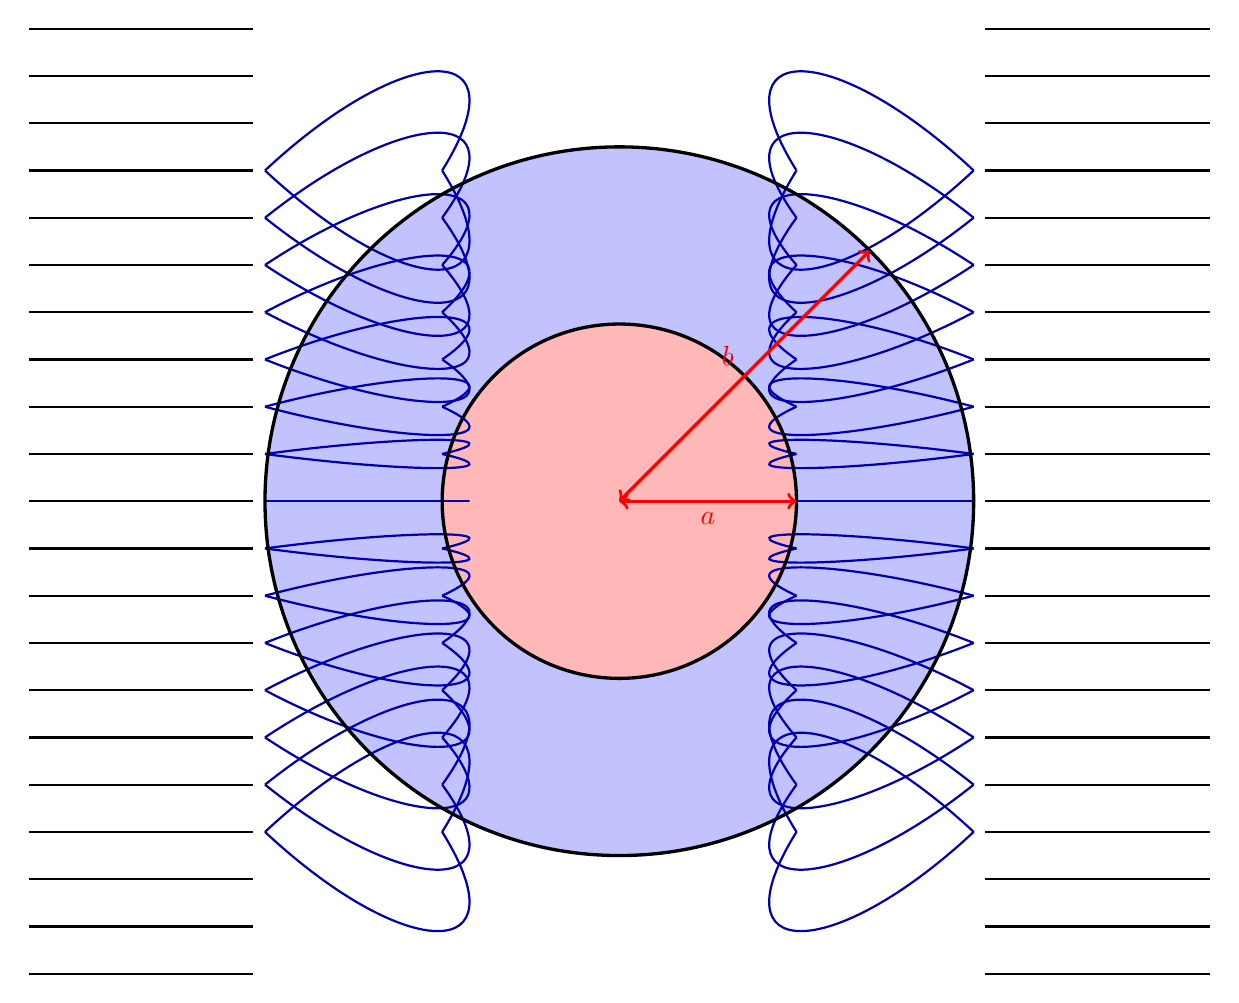
\begin{tikzpicture}[scale=1.5]
  
  % Define radii
  \def\ra{1.5}  % inner radius a
  \def\rb{3}    % outer radius b
  
  % Fill the regions
  \fill[blue!40, opacity=0.6] (0,0) circle (\rb);
  \fill[white] (0,0) circle (\ra);
  \fill[red!40, opacity=0.7] (0,0) circle (\ra);
  
  % Draw straight lines on the left (before cloak)
  \foreach \y in {-4,-3.6,...,4} {
    \draw[thick] (-5,\y) -- (-\rb-0.1,\y);
  }
  
  % Draw straight lines on the right (after cloak)
  \foreach \y in {-4,-3.6,...,4} {
    \draw[thick] (\rb+0.1,\y) -- (5,\y);
  }
  
  % Draw curved flow lines around the cloak
  \foreach \y in {-2.8,-2.4,-2.0,-1.6,-1.2,-0.8,-0.4,0,0.4,0.8,1.2,1.6,2.0,2.4,2.8} {
    % Calculate control points for bezier curves
    \pgfmathsetmacro{\yshift}{0.4*abs(\y)}
    
    % Upper curve (left half)
    \draw[thick, blue!70!black] 
      (-\rb,\y) .. controls (-1.8,{\y+\yshift}) and (-0.8,{\y+\yshift}) .. (-\ra,\y);
    
    % Upper curve (right half)
    \draw[thick, blue!70!black] 
      (\ra,\y) .. controls (0.8,{\y+\yshift}) and (1.8,{\y+\yshift}) .. (\rb,\y);
    
    % Lower curve (left half)
    \draw[thick, blue!70!black] 
      (-\rb,\y) .. controls (-1.8,{\y-\yshift}) and (-0.8,{\y-\yshift}) .. (-\ra,\y);
    
    % Lower curve (right half)
    \draw[thick, blue!70!black] 
      (\ra,\y) .. controls (0.8,{\y-\yshift}) and (1.8,{\y-\yshift}) .. (\rb,\y);
  }
  
  % Draw the boundaries
  \draw[very thick, black] (0,0) circle (\rb);
  \draw[very thick, black] (0,0) circle (\ra);
  
  % Add dimension labels
  \draw[<->, red, very thick] (0,0) -- (\ra,0) node[midway, below] {$a$};
  \draw[<->, red, very thick] (0,0) -- ({0.707*\rb},{0.707*\rb}) 
    node[midway, above left] {$b$};
  
\end{tikzpicture}
% \end{document}
